Las personas usan latitudes (las líneas horizontales) y las longitudes (las líneas verticales) en el sistema de coordenadas de la Tierra. La longitud avanza en intervalos desde $0$ grados (Greenwich) hasta $+180^0$ * hacia el este y $-180^0$ * hacia el oeste. La latitud avanza en intervalos desde 0 grados (el Ecuador) para $+90^0$ * (hacia el Polo Norte) y $-90^0$ * (hacia el Polo Sur). 

La pregunta más interesante es: cual es la distancia / geográfica esférica entre  dos ciudades ($p$ y $q$) en tierra con radio $r$, denotada de por ($p_{lat}$,$p_{long}$) y ($q_{lat}$,$q_{long}$). Todas las coordenadas están en radianes. (o sea el rango del $-180 \dots 180$ del converso de longitud y $-90 \dots 90$ se extienden de latitudes para $-\Pi  \dots \Pi$ y $-\frac{\Pi}{2}  \dots \frac{\Pi}{2}$ respectivamente.

La fórmula de distancia esférica utiliza la fórmula del coseno para calcular la distancia entre dos puntos en la superficie esférica, teniendo en cuenta la curvatura de la esfera. Esta fórmula tiene en cuenta las coordenadas geográficas de los dos puntos, es decir, sus latitudes y longitudes en radianes.

La fórmula del coseno utiliza la función arcocoseno para calcular la distancia esférica entre los dos puntos, teniendo en cuenta la diferencia en las latitudes y longitudes de los puntos. La fórmula tiene en cuenta la curvatura de la esfera al calcular la distancia entre los dos puntos, lo que la hace más precisa que simplemente usar la distancia euclidiana en un plano. Sea una esfera sólida de centro $O$ y radio $r$ como se muestra en la figura siguiente: 

% TODO: \usepackage{graphicx} required
\begin{figure}[h!]
	\centering
	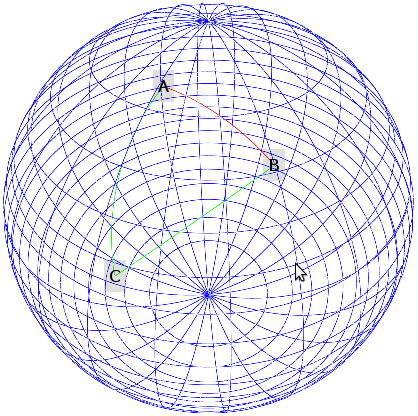
\includegraphics[width=0.3\linewidth]{img/esfera}
	\label{fig:esfera}
\end{figure}

y dos puntos $A=(x_0;y_0)$ y $B=(x_1;y_1)$ localizados sobre la superficie de la esfera, donde $x_i$, $y_i$ son coordenadas esféricas definidas como las amplitudes de los ángulos de longitud y latitud respectivamente. 

Sea la esfera de centro en el origen de coordenadas $O$ y radio $r$ y dos puntos superficiales Punto $A=(\alpha_A;\beta_A)$ y Punto $B=(\alpha_B;\beta_B)$ donde $ \alpha_A,\alpha_B \in [-\pi,\pi]$ son las longitudes de sus respectivos puntos respecto al eje x;$ \beta_A,\beta_B \in [-\frac{\pi}{2},\frac{\pi}{2}]$ son las latitudes correspondientes de $A$ y $B$. 

Traducidos a coordenadas euclideanas en el espacio los puntos $A=(x_A;y_A;z_A)=(r\cdot \cos \alpha_A \cdot \cos \beta_A; r \cdot \sin \beta_A; r \cdot \sin \alpha_A \cdot \cos \beta_A)$  y $B=(x_B;y_B;z_B)=(r\cdot \cos \alpha_B \cdot \cos \beta_B; r \cdot \sin \beta_B; r \cdot \sin \alpha_B \cdot \cos \beta_B)$ ; puede calcularse la longitud de la cuerda relativa a la ortodrómica que ambos conforman: 

$$d(A,B) = \sqrt{(B_x-A_x)^2+(B_y-A_y)^2+(B_z-A_z)^2} $$

Luego la amplitud del arco correspondiente a ese segmento es: 

$$\angle AOB = \arccos(\frac{2 \cdot r^2 - d(A,B)^2}{2 \cdot r^2})$$

Asumiendo que la función arcoseno devuelve la amplitud del ángulo en radianes. Uniendo todo, la expresión completa de la distancia esférica entre dos puntos dadas sus coordenadas esféricas queda: 

$$d_s(A,B,r) = \angle AOB \cdot r = r \cdot \arccos ( \frac{2\cdot r^2 - (x_B-x_A)^2 - (y_B-y_A)^2 - (z_B-z_A)^2}{2\cdot r^2} )$$

